\documentclass[a4paper,12pt]{article}

\usepackage[utf8]{inputenc}
\usepackage{graphicx}
\usepackage[table]{xcolor}
\usepackage{pdfpages}
\usepackage{hyperref}
\usepackage{float}
\usepackage[top=1in, bottom=1.25in, left=1in, right=1in]{geometry}
\usepackage{wrapfig}
\usepackage{enumitem}
\usepackage{gensymb}
\usepackage{fancyref}
\usepackage{fancyhdr}
\usepackage{amssymb}
\usepackage{supertabular}
\usepackage{textcomp}
\usepackage{gensymb}
\usepackage{wallpaper}
\usepackage{rotating}
\usepackage{xspace}

\pagestyle{fancy}
%\lfoot{Copyright 2020 Sa\v so Kiselkov}

\renewcommand{\familydefault}{\sfdefault}

\definecolor{lightgrey}{rgb}{0.9, 0.9, 0.9}
\definecolor{grey}{rgb}{0.67, 0.67, 0.67}
\definecolor{darkgrey}{rgb}{0.2, 0.2, 0.2}
\definecolor{tablehdrcolor}{rgb}{0.9, 0.9, 1.0}
\definecolor{tablecontcolor}{rgb}{0.95, 0.95, 0.95}
\definecolor{noteboxcolor}{rgb}{.98, 0.8, 0}
\definecolor{warnboxcolor}{rgb}{0.96, 0.15, 0.15}

\newcommand{\filetext}[1]{\vspace{.5em}%
\noindent\hspace{0.05\textwidth}\fcolorbox{black}{lightgrey}{%
\parbox{0.9\textwidth}{\texttt{#1}}}%
\vspace{.5em}}

\newcommand{\notebox}[1]{\vspace{.5em}%
\noindent\hspace{0.05\textwidth}\fcolorbox{black}{noteboxcolor}{%
\parbox{0.9\textwidth}{{\large\bf NOTE}\vspace{.35em}\hrule\vspace{.25em}#1}}%
\vspace{.5em}}

\newcommand{\warnbox}[1]{\vspace{.5em}%
\noindent\hspace{0.05\textwidth}\fcolorbox{black}{warnboxcolor}{%
\parbox{0.9\textwidth}{{\large\bf WARNING!}\vspace{.35em}\hrule%
\vspace{.25em}#1}}\vspace{.5em}}

\newcommand{\myfrac}[2]{%
\textsuperscript{#1}\hspace{-0.4em}$\diagup$\hspace{-0.4em}\textsubscript{#2}}

\newcommand{\fileicon}[1]{\raisebox{-.15em}%
{\includegraphics[height=.9em]{../src/#1}}}

\newcommand{\libcpdlc}{\textbf{libcpdlc}\xspace}

\setlist{nolistsep}

\setlength{\abovecaptionskip}{0pt}
\setlength{\belowcaptionskip}{0pt}
\setlength\intextsep{0pt}

\overfullrule=2cm

\title{libcpdlc Wire Format Guide}
\author{Sa\v so Kiselkov}

\begin{document}

\thispagestyle{empty}

\vspace*{25em}
\begin{center}
\resizebox{0.5\linewidth}{!}{libcpdlc}\\
\strut\\
{\Large Wire Format Guide}
\end{center}
\vspace{21em}
Version: 1.0

\newpage

\tableofcontents

\newpage

\ThisCenterWallPaper{1.02}{warn_pattern.eps}
\thispagestyle{empty}

\section{LICENSE \& DISCLAIMER}

Permission is hereby granted, free of charge, to any person obtaining a
copy of this software and associated documentation files (the
"Software"), to deal in the Software without restriction, including
without limitation the rights to use, copy, modify, merge, publish,
distribute, sublicense, and/or sell copies of the Software, and to permit
persons to whom the Software is furnished to do so, subject to the
following conditions:

\strut

\noindent The above copyright notice and this permission notice shall be
included in all copies or substantial portions of the Software.

\strut

\noindent THE SOFTWARE IS PROVIDED "AS IS", WITHOUT WARRANTY OF ANY KIND,
EXPRESS OR IMPLIED, INCLUDING BUT NOT LIMITED TO THE WARRANTIES OF
MERCHANTABILITY, FITNESS FOR A PARTICULAR PURPOSE AND NONINFRINGEMENT. IN
NO EVENT SHALL THE AUTHORS OR COPYRIGHT HOLDERS BE LIABLE FOR ANY CLAIM,
DAMAGES OR OTHER LIABILITY, WHETHER IN AN ACTION OF CONTRACT, TORT OR
OTHERWISE, ARISING FROM, OUT OF OR IN CONNECTION WITH THE SOFTWARE OR THE
USE OR OTHER DEALINGS IN THE SOFTWARE.

\newpage

\section{Overview}

\noindent\libcpdlc is a generic and open-source implementation of the
CPDLC protocol as specified in the ICAO GOLD document. To facilitate
maximum interoperability, the \libcpdlc system doesn't rely on any
proprietary software or standards and is instead defined using only
Internet-standard methods.

\noindent The line protocol specification of \libcpdlc consists of two
fundamental layers:

\begin{itemize}

\item The base connection layer is intended to simulate an abstract
Aeronautical Telecommunication Network (ATN). Since \libcpdlc doesn't
make any assumptions about the exact method of transport used to transfer
CPDLC messages, the ATN is simulated simply as an plain TLS connection
between \libcpdlc clients and the \libcpdlc server.

The server assumes the role of providing the base transfer layer of
messages between \libcpdlc clients. The server also provides automatic
message buffering and delayed delivery. In addition, the server provides
a secondary layer of security to prohibit "bad faith actors" from
submitting malformed messages, overloading the network with spam or
communicating with unapproved 3rd parties via the network.

\item The CPDLC messaging layer. This is transported on top of the
virtual ATN network. The format of these messages utilizes plain ASCII
text and URL escaping to allow transfer of non-alphanumerical characters.

Once connected and authenticated, all clients sit on one big virtual ATN,
each identified by a unique callsign identifier. This can be an arbitrary
sequence of letters and numbers, but will typically be the flight number
or tail number for aircraft stations, or a fixed station identifier for
an ATC station.

\end{itemize}

\newpage

\section{TLS Connection}

As mentioned in the previous section, \libcpdlc operates over a TLS
socket connection. \libcpdlc was designed around a "secure-by-default"
philosophy and as such there is no unencrypted mode of operation. At a
minimum, the \libcpdlc server's certificate must be authenticated by the
\libcpdlc clients. There are no specific requirements on the certificate
structures used by a particular \libcpdlc deployment.

\begin{center}
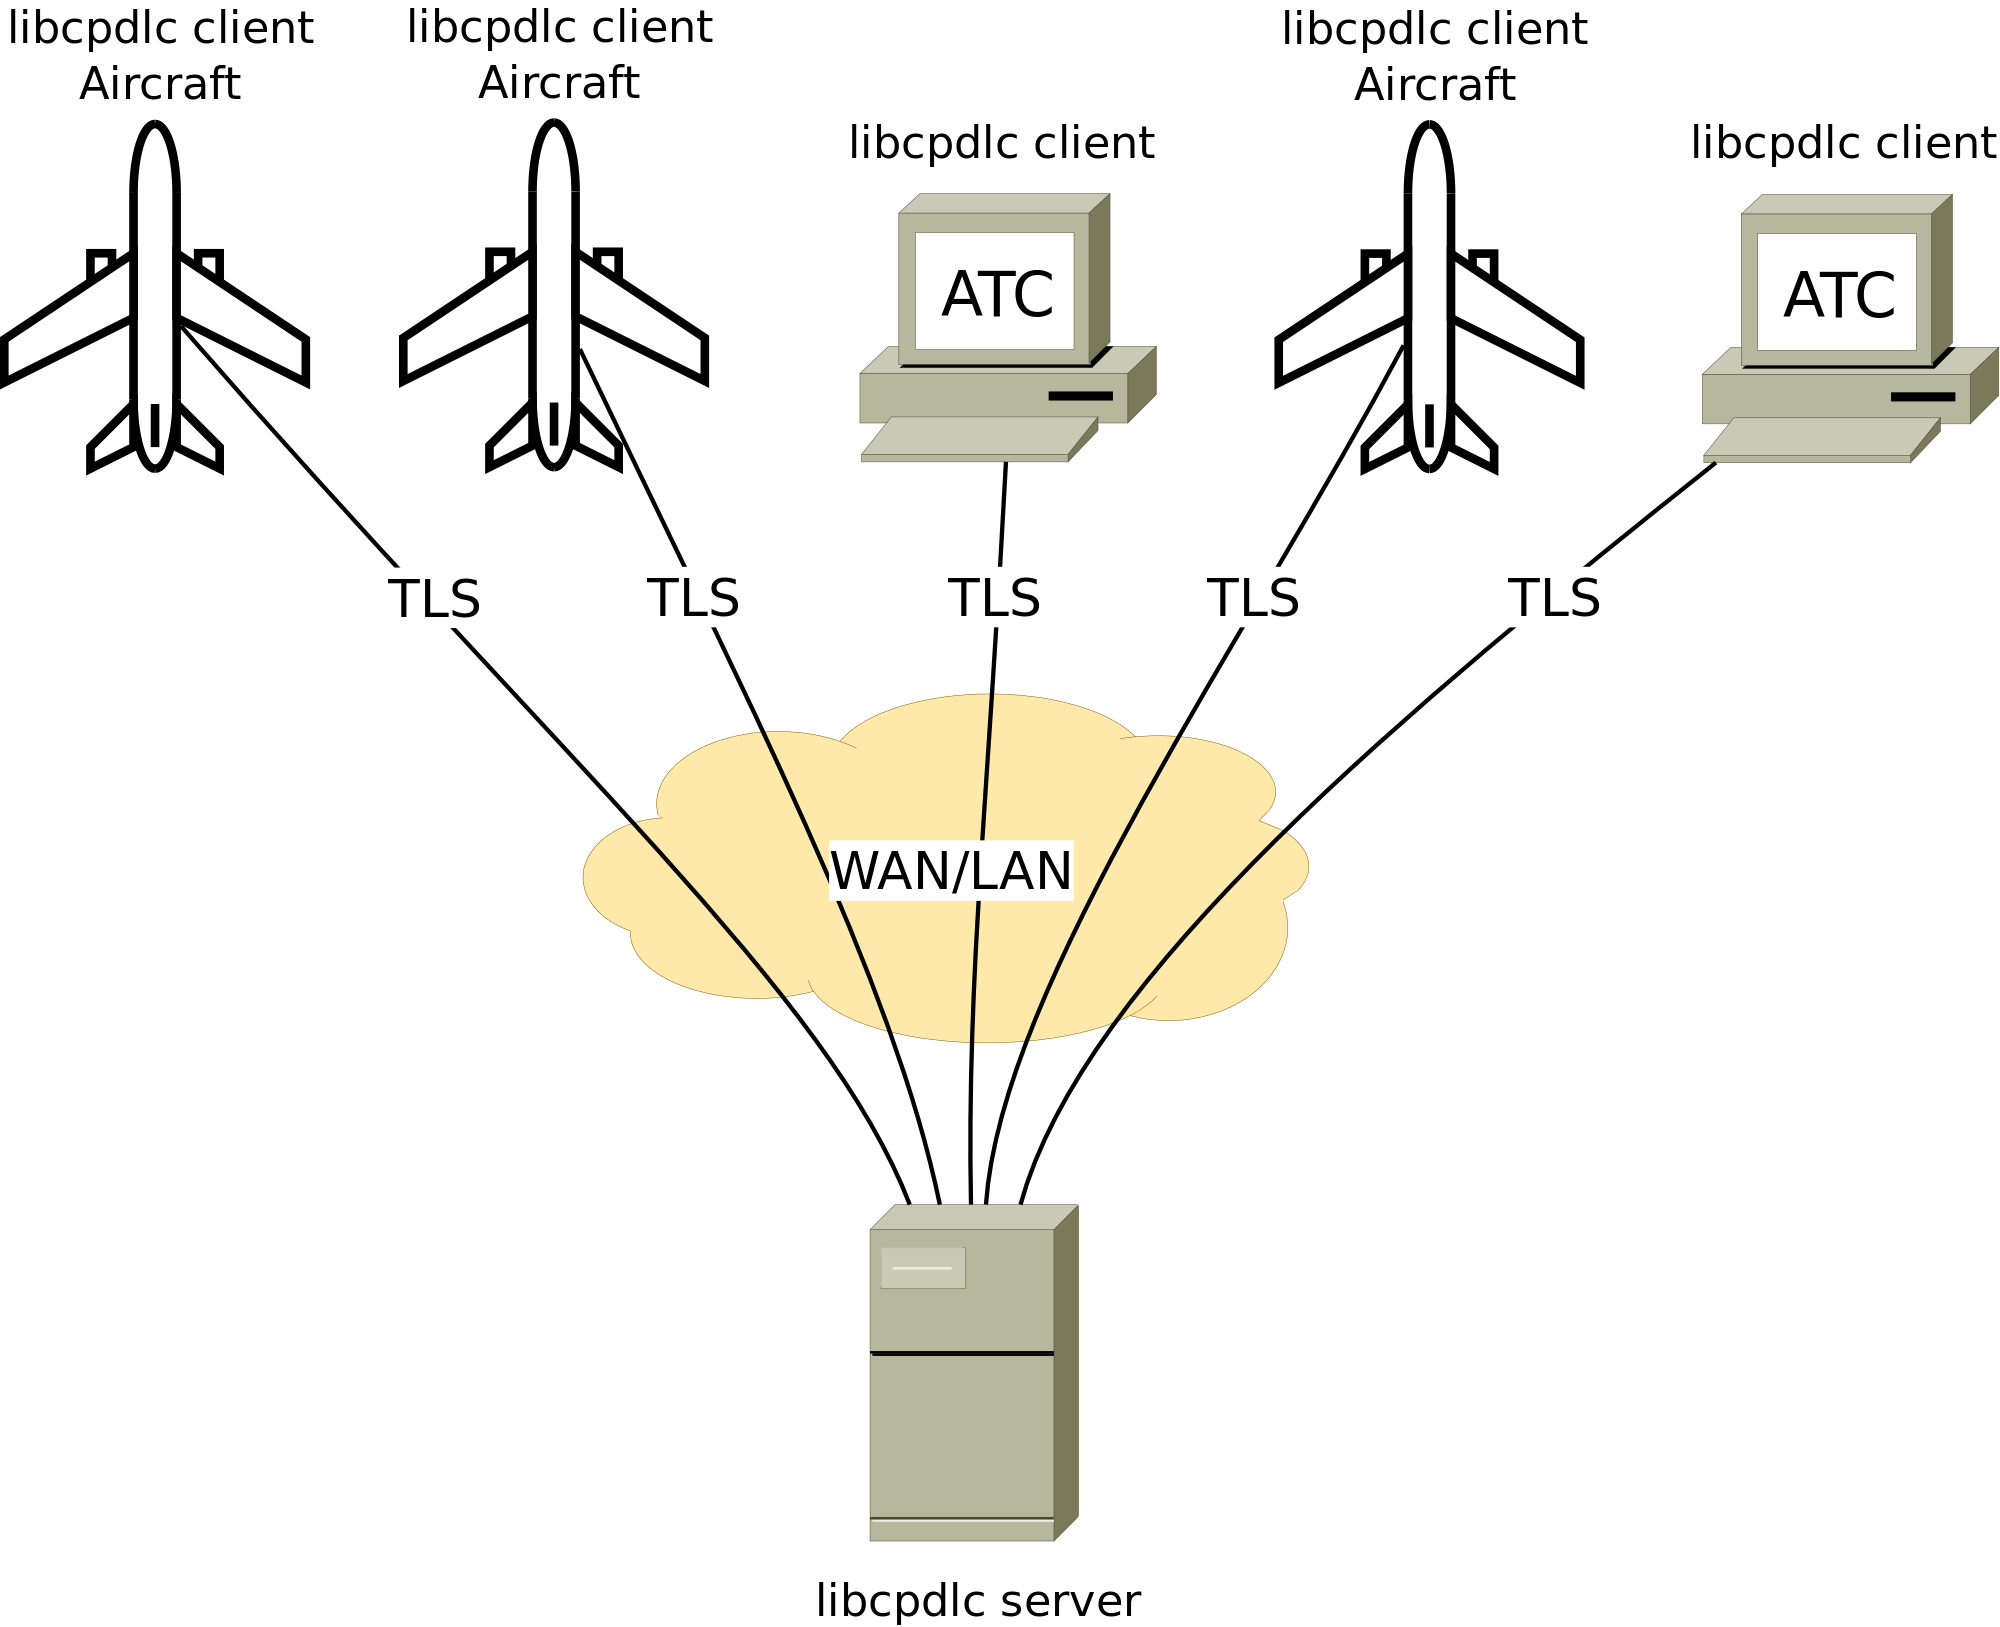
\includegraphics[width=0.85\textwidth]{base_network.png}
\end{center}

\noindent Here we will list some common ways that a \libcpdlc deployment
might be configured:

\begin{itemize}

\item By default, the \libcpdlc client library will verify that the
server's connection hostname (or IP address) matches the {\em Common
Name} or {\em Subject Alt Name} fields in the server certificate. The
validity of the server certificate is verified against a list of trusted
Certificate Authorities (CA). This list can be supplied by the software
integrating \libcpdlc, or it can be automatically retrieved from the
operating system's trusted CA pool (on operating systems where such a
mechanism is available).

If the deployment requires more strict checking of the server identity,
the client software should provide a very restrictive list of trusted CAs
(most likely only a single one). Combined with the security mechanisms in
the TLS protocol, this effectively eliminates any potential for server
spoofing.

\item The \libcpdlc server can also be configured to require the client
to submit its own certificate. All of the CA checks that are available to
the client, are also available to the server. Client certificates can be
utilized to implement security mechanisms such as:

\begin{itemize}

\item API keys: in this mechanism, only a limited set of trusted client
software is ever allowed to connect to the server. The server's operator
controls and hands out client certificates, which are embedded in the
client software. The \libcpdlc client library allows passing encrypted
private key data together with a decryption key to the embedded TLS
library. This way, the private key and certificate of the client software
isn't exposed to trivial forms of debugging analysis. The server operator
can issue a new API key when integrating a new client, and optionally
revoke any compromised API keys.

\item Individual end-user keys: the \libcpdlc server can simply validate
that the client was issued a personal, non-revoked certificate by the
server's operator. The server can optionally also pass the certificate's
{\em Distinguished Name} field to an external authenticator application
to execute additional validation checks.

\end{itemize}

\item As an additional security measure, the server also allows the
use of IP address whitelists and blacklists (including subnet masking).
If an IP address is not found on the whitelist (when in use), or is found
on the blacklist, the connection attempt is rejected before even TLS
handshake initiation. This security measure can be used to help deal with
persistent spammers and/or denial-of-service attackers.

\end{itemize}

\noindent Once the initial TLS handshake is completed, the \libcpdlc
server gives the client a 30 second grace period during which the client
must send a valid LOGON CPDLC message to connect to an ATC station known
to the server. If this doesn't happen in the allotted time, the server
terminates the connection.

\newpage

\section{CPDLC Messaging}

The CPDLC network is inherently designed around many-to-one
communication.

\begin{itemize}

\item During a LOGON, aircraft stations must supply a ``TO'' field in
their LOGON message to the server. This ties the aircraft station to a
single destination ATC station. Subsequent messages from aircraft
\textbf{must not} specify a ``TO'' field. The \libcpdlc server infers the
destination of their messages from their active LOGON. The aircraft
station isn't permanently tied to a single LOGON. It can send a LOGOFF
message and subsequently LOGON to a different ATC station. However, at
any given time, an aircraft station can only be logged onto a single ATC
station.

\item ATC stations LOGON to the server to establish their identity
and their role as ATC. While this isn't a realistic representation of the
CPDLC data flow, the LOGON mechanism is simply reused for ATC stations to
establish client-server trust over an untrustworthy network. When sending
CPDLC messages, ATC stations must explicitly tell the server which
aircraft station they wish to communicate with in every message they
submit.

\end{itemize}

\noindent Stations are identified by a unique sequence of letters or
numbers. These will typically be 4-letter ICAO ATC station IDs, or
aircraft flight number/tail number for aircraft stations.

The \libcpdlc server provides automatic message buffering. If the
destination station of a message isn't currently connected to the server,
the server will buffer the message up to a message-type-dependent
timeout. Since the server understands the CPDLC protocol, it will
automatically drop undelivered messages after the timeout has expired.
The sending station should keep track of its own message response
timeouts and also mark the message as being expired.

\begin{center}
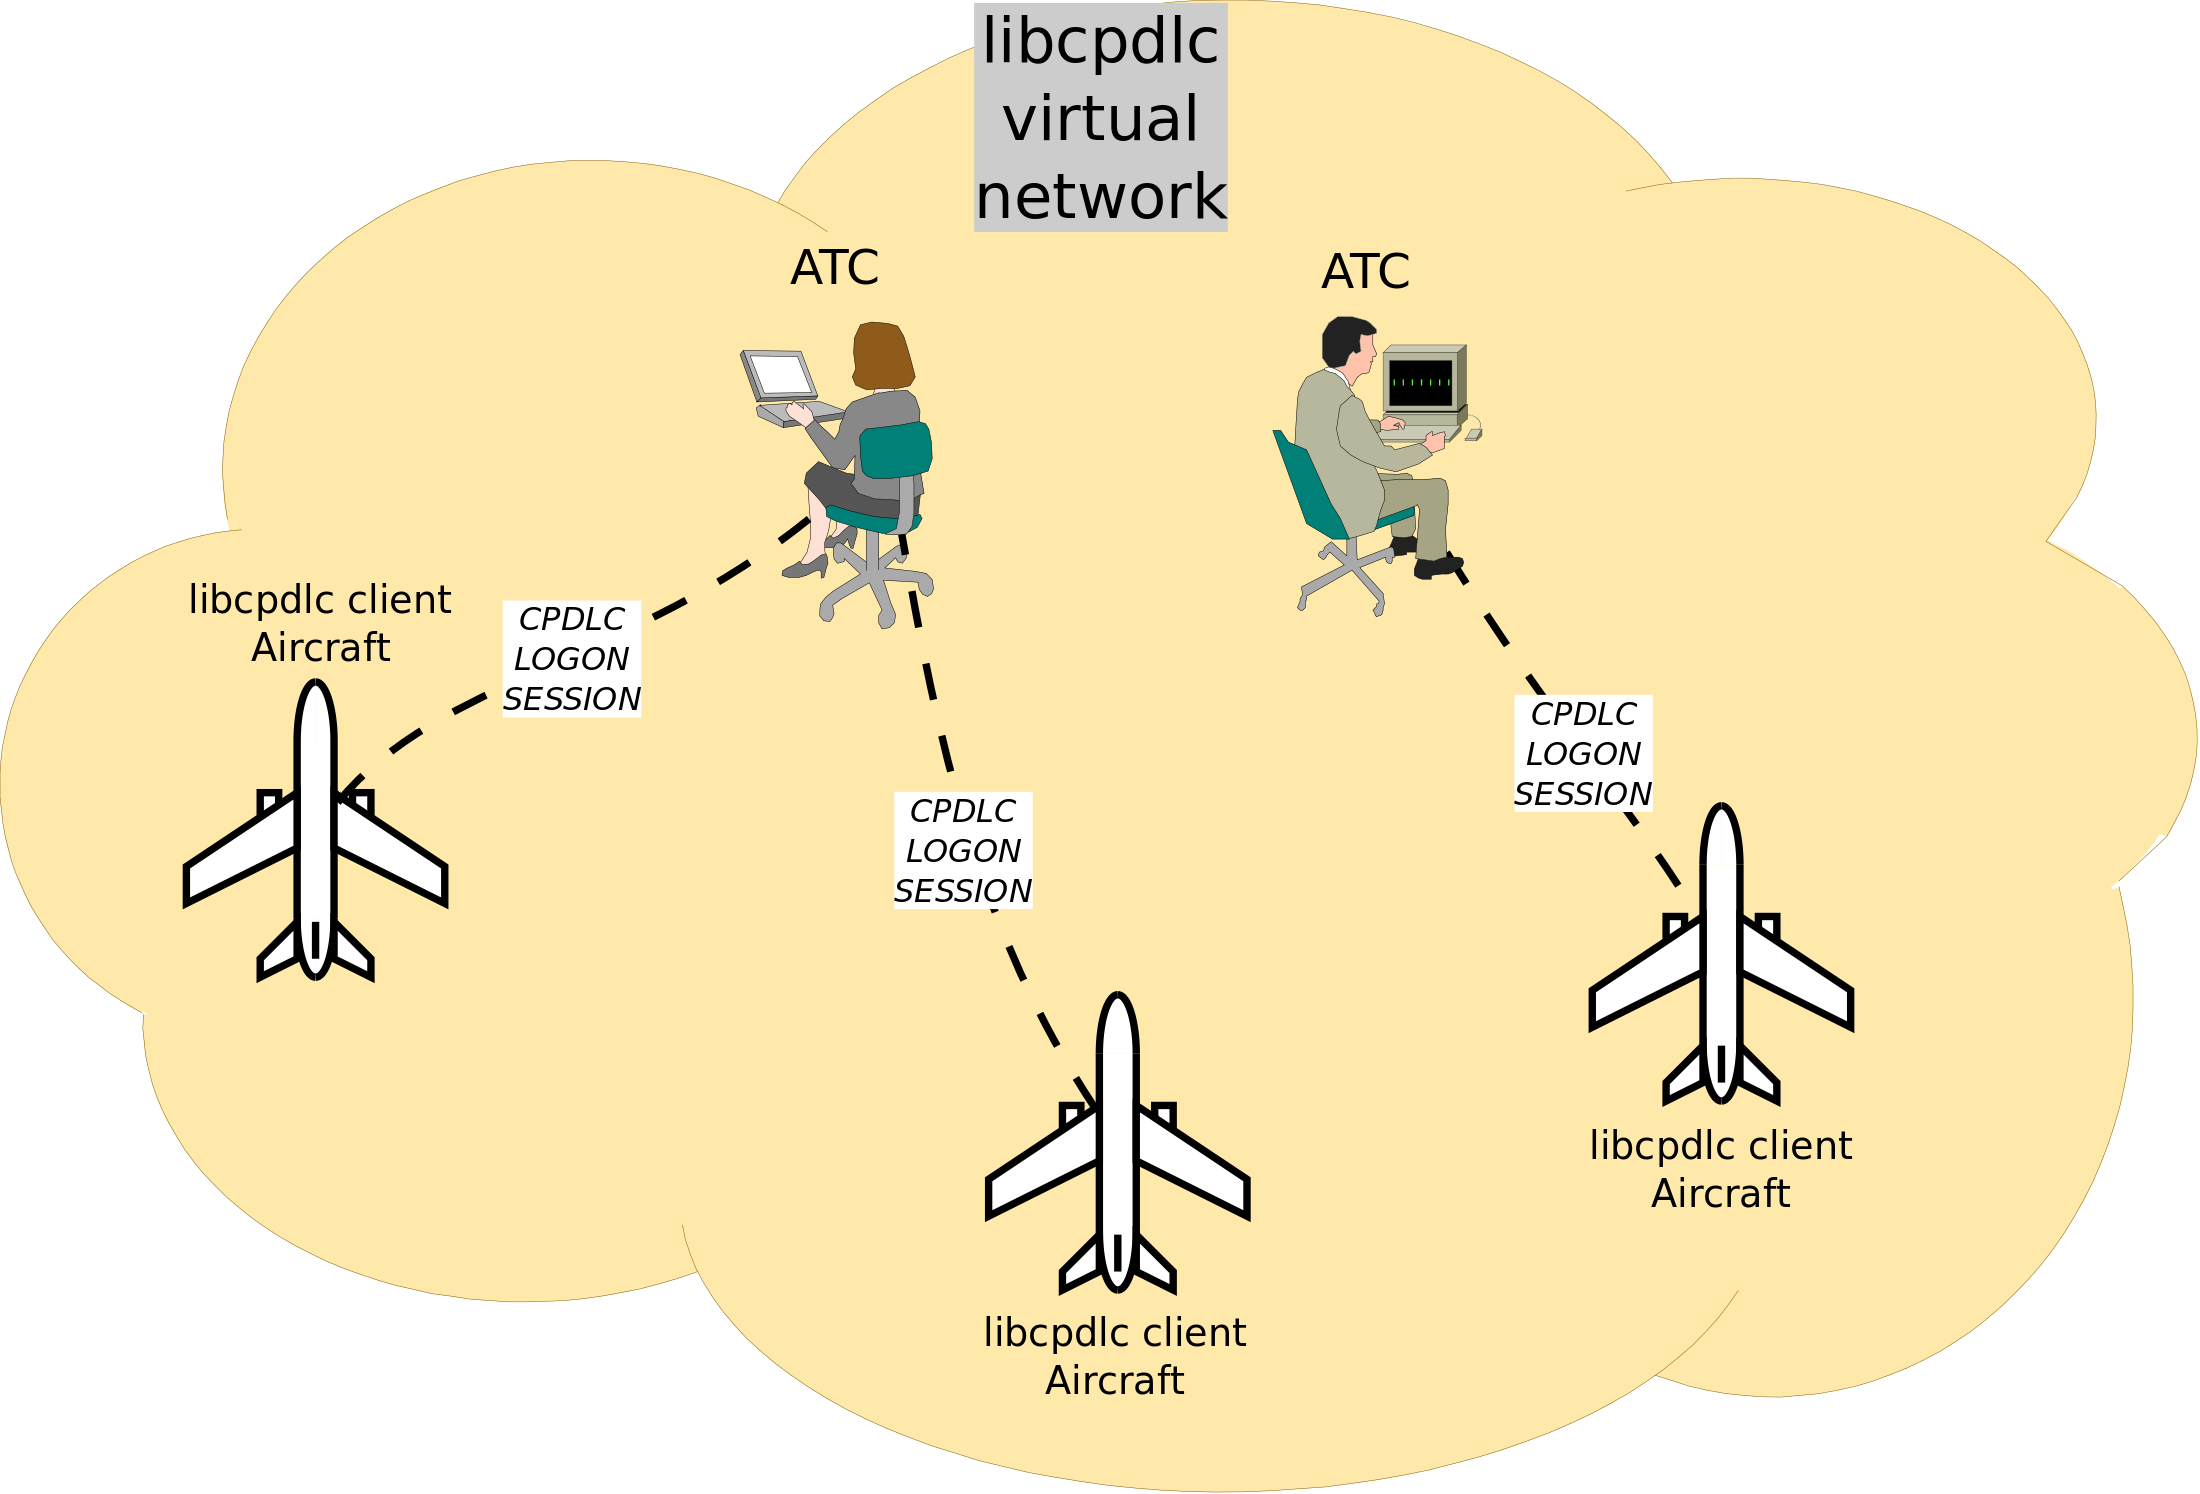
\includegraphics[width=0.85\textwidth]{virt_net.png}
\end{center}

\subsection{CPDLC Message Format}

Each CPDLC message consists of a single plain-text line of ASCII-encoded
characters, terminated by a single Line Feed (LF, 0x10) character. This
character is denoted using the \texttt{\textbackslash n} escape sequence
in the sample printouts below. The message is internally subdivided into
NAME=VALUE pairs, delimited by a single slash '/' character, as follows:

\begin{verbatim}
PKT=CPDLC/NAME1=VALUE1/NAME2=VALUE2...\n
\end{verbatim}

\noindent In some messages, the VALUE portion of a pair can be omitted if
the NAME by itself clearly communicates intent.

Sometimes the message requires the encoding of non-alphanumeric
characters, such as embedded newline characters, or whitespace that
is intended to appear as part of a single message component. In that
case, URL-escaping of the character is utilized:

\begin{verbatim}
PKT=CPDLC/MIN=10/MRN=0/TO=N123AB/MSG=UM160 KZAK OAKLAND%20OCEANIC\n
\end{verbatim}

\noindent In the example message above, the full name of the ATC station
contains a space, which must be preserved in the name. The escape
sequence \textbf{\%20} denotes that the character that should be
substituted in its place is ASCII character 0x20 hexadecimal (a space
character).

\subsection{Message MIN and MRN numbers}
\label{MinMrn}

The CPDLC protocol requires that messages have a unique number associated
with them for the purposes of message thread tracking.

\begin{description}

\item[MIN] -- Message Identification Number. This number uniquely
identifies the message in the message flow between the aircraft and ATC
stations. Each side of a connection keeps its own incrementing message
number counter. After sending every message, the MIN counter is
incremented, thus assuring that subsequent messages receive a unique
identifier. Identifiers shouldn't be reused within a within a single
LOGON session, otherwise there is a risk of confusion when matching
responses to requests.

\item[MRN] -- Message Response Number. Whenever a response message is
generated, the original message's MIN number is embedded in the MRN field
of the responses. The response message also gets its own unique MIN
generated. Using the MRN, the response can be matched to the original
message which triggered the response.

\end{description}

\noindent Example of MIN/MRN pairing:

\begin{enumerate}

\item Aircraft station submits the following request altitude request:

\begin{verbatim}
PKT=CPDLC/MIN=10/MSG=DM6 FL350\n
\end{verbatim}

\item The ATC station responds with a STANDBY. The MRN field is set
to the MIN field of the original message to clearly tie the STANDBY
message to the altitude request:

\begin{verbatim}
PKT=CPDLC/MIN=25/MRN=10/FROM=KZAK/MSG=UM1\n
\end{verbatim}

\end{enumerate}

\subsection{CPDLC LOGON}

Once connected by a TLS connection to the \libcpdlc server, the client
\textbf{must} send a valid LOGON message within 30 seconds. The LOGON
message has the following format:

\begin{verbatim}
PKT=CPDLC/LOGON=[SECRET]/FROM=[ORIGIN]/[TO=DEST]/MIN=0\n
\end{verbatim}

\noindent The LOGON message is special and is recognized by the \libcpdlc
server. As such, it is NOT forwarded to any other station. Instead, it is
used by the \libcpdlc server to establish the client's identity.

The server performs an authentication check by passing the contents of
the FROM and LOGON fields to an external authenticator. This
authenticator must respond with a simple two-line response that
informs the \libcpdlc server whether the station is:

\begin{enumerate}

\item The first line informs the server whether to permit the LOGON. If
the response is `1', the client is allowed to assume the identity
contained within the ``FROM'' field. If the response is `0', the LOGON
request is rejected and the client remains un-authenticated. It must
submit a valid LOGON request within the next 30 seconds, or the server
will terminate the connection.

\item The second line informs the server whether the client is an ATC
station, or an aircraft station. If the authenticator returns `1', the
client assumes the role of ATC and conversely if it returns `0', the
client assumes the role of an aircraft. The \libcpdlc server uses this
information to provide message integrity checking, as well as
automatically routing aircraft message to the target ATC station.

\end{enumerate}

\noindent The ``TO'' field \textbf{must} be provided by aircraft stations
to denote which ATC station they wish to LOGON to. Conversely, ATC
stations \textbf{must not} provide this information in the LOGON message.
They will instead stamp each message they send with a ``TO'' field, which
informs the \libcpdlc server which aircraft station they are intended
for. If the intended aircraft station isn't currently connected to the
server, the server will buffer the message up to a certain
message-type-determined timeout before dropping it.

\noindent When a LOGON is successful, the \libcpdlc server itself
directly responds to the LOGON message as follows:

\begin{verbatim}
PKT=CPDLC/LOGON=SUCCESS/FROM=ATN/MIN=0/MRN=0\n
\end{verbatim}

\noindent Conversely, if the LOGON failed, the server responds as
follows:

\begin{verbatim}
PKT=CPDLC/LOGON=FAILURE/FROM=ATN/MIN=0/MRN=0\n
\end{verbatim}

\subsubsection{ATC LOGON}

As a special case, ATC stations are permitted to have multiple active
LOGON sessions as multiple identities. This is used for cases where a
client needs to multiplex several ATC station identifiers (e.g.\ an
air traffic controller working multiple sectors). The ATC station can
drop an existing LOGON identity by sending a matching LOGOFF message,
or assume new identities after connecting by sending more valid LOGON
messages with different ``FROM'' fields.

\subsection{CPDLC LOGOFF}

When a client wishes to terminate its session with the ATN, it sends
a LOGOFF message:

\begin{verbatim}
PKT=CPDLC/LOGOFF/MIN=20\n
\end{verbatim}

\noindent This message is intercepted and processed by the \libcpdlc
server itself. The server releases the client's identity and stops
accepting CPDLC messages from the client until another valid LOGON is
received.

The server also recognizes uplink message 161 ({\em End Service}) when
sent by an ATC station to an aircraft station. It serves as an
ATC-initiated LOGOFF. If preceded at an earlier time by uplink message
160 ({\em Next Data Authority}), the aircraft station can use this
condition to automate logging onto the next ATC station in sequence:

\begin{enumerate}

\item Aircraft receives the {\em Next Data Authority} message from the
Current Data Authority:

\begin{verbatim}
PKT=CPDLC/MIN=10/TO=N123AB/MSG=UM160 KZAK OAKLAND%20OCEANIC\n
\end{verbatim}

\item Shortly thereafter, the current ATC station terminates the LOGON by
sending an End Service message:

\begin{verbatim}
PKT=CPDLC/MIN=11/TO=N123AB/MSG=UM161\n
\end{verbatim}

\item Upon receipt of the {\em End Service} message, the aircraft station
initiates a new LOGON to the next data authority:

\begin{verbatim}
PKT=CPDLC/LOGON=[SECRET]/FROM=N123AB/TO=KZAK/MIN=22\n
\end{verbatim}

\item The \libcpdlc server responds with a LOGON SUCCESS message:

\begin{verbatim}
PKT=CPDLC/LOGON=SUCCESS/FROM=ATN/MIN=0/MRN=22\n
\end{verbatim}

\end{enumerate}

\begin{center}
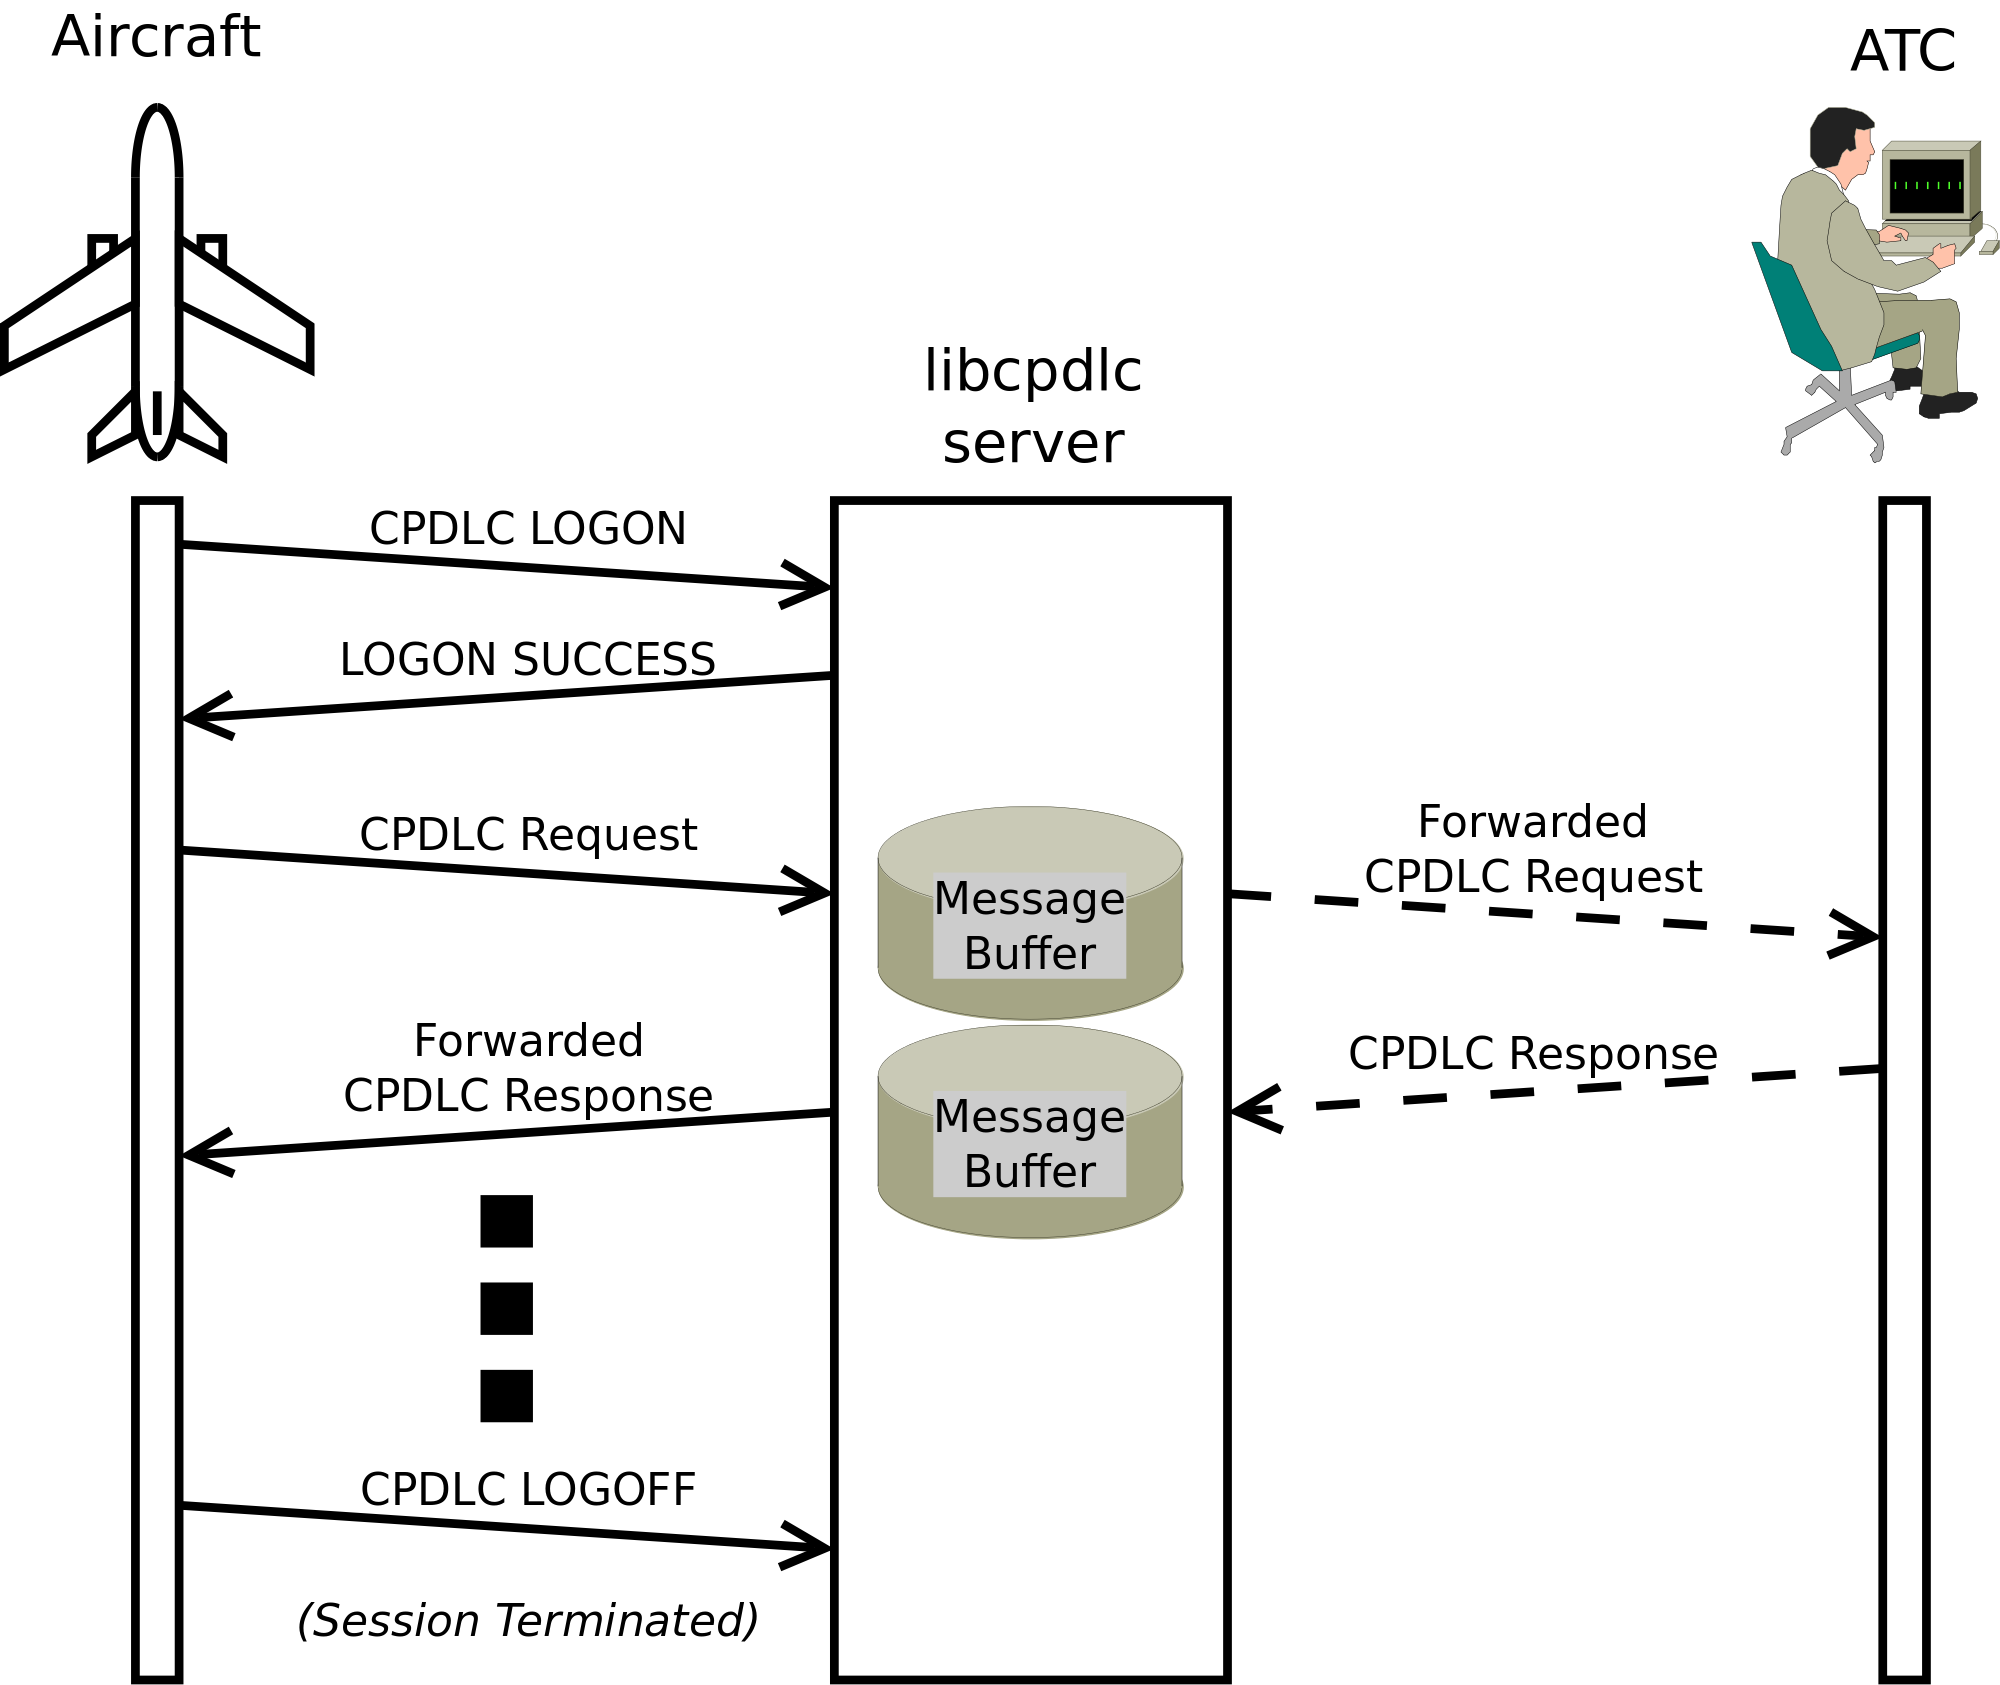
\includegraphics[width=0.75\textwidth]{logon_flow.png}
\end{center}

\section{CPDLC Messages}

Every subsequent CPDLC message sent after a successful LOGON conforms to
the following format:

\begin{verbatim}
PKT=CPDLC/MIN=<MIN>/[MRN=<MRN>]/[FROM=<ID>]/[TO=<ID>]/MSG=<msg body>\n
\end{verbatim}

\begin{description}

\item[MIN] -- unique message identification number. See section
\ref{MinMrn} for more information on message numbering.

\item[MRN] -- only used on messages responding to other messages.

\item[FROM] -- only used by ATC stations. ATC clients can assume multiple
station identities and as such must disambiguate the station identity
from which a particular message was sent. Aircraft stations will only
ever see the ``FROM'' field on messages they are receiving. If they
attempt to include a ``FROM'' field in their messages, the \libcpdlc
server will reject the message.

\item[TO] -- must only be specified on messages from ATC stations
to identify which aircraft station they wish the message to be delivered
to. Aircraft station messages don't use this field, since the destination
of their messages is automatically derived from their active LOGON. The
\libcpdlc server also automatically stamps this field onto aircraft
messages, so the ATC client can disambiguate which ATC station the
aircraft wishes to communicate with.

\item[MSG] -- actual message body of whitespace separated elements. The
contents of this field are message-type dependent. Extra whitespace
between message arguments will be ignored.

\end{description}

\noindent The remainder of this section describes the contents of the
message body.

\subsection{Message Type Header}

Every message body must start with a message type header:

\begin{description}

\item[UMxx] -- Uplink Message, where `xx' denotes a number from the CPDLC
uplink message list. The \libcpdlc server verifies that only ATC stations
attempt to send uplink messages, as well as that any additional required
message parts are present and correctly formatted.

\item[DMxx] - Downlink Message, where `xx' denotes a number from the
CPDLC downlink message list. As before, the \libcpdlc server verifies
that downlink messages are only sent by aircraft stations and that they
are correctly formatted.

\end{description}

\subsection{Message Arguments}

A number of messages take additional arguments. A complete list will be
provided in a later section. However, all of the arguments are formatted
consistently according to the type of information they contain.

\begin{description}

\item[Fulltext] -- any fulltext argument is encoded as a single
contiguous string of alphanumeric characters. Escape sequences are used
in places where whitespace in the freetext body would cause ambiguities
in the message encoding. Example encoding of a freetext downlink message
containing the string ``HELLO WORLD!'':

\begin{verbatim}
PKT=CPDLC/MIN=1/MSG=DM67 HELLO%20WORLD%21\n
\end{verbatim}

\item[Altitude] -- altitudes are encoded in one of the following formats:

\begin{itemize}

\item Altitude in feet (QNH): 3-5 digits denoting the altitude in
units of feet. Example climb instruction message to an altitude of 12000
feet:

\begin{verbatim}
PKT=CPDLC/MIN=60/MSG=UM20 12000\n
\end{verbatim}

\item Altitude as a flight level (QNE): the letters `FL' followed by 1-3
digits, denoting the level in hundreds of feet. Example climb instruction
message to flight level 350:

\begin{verbatim}
PKT=CPDLC/MIN=60/MSG=UM20 FL350\n
\end{verbatim}

\item Metric altitude (QNH): 3-5 digits denoting the altitude in units
of meters, followed by the letter `M'. Example climb instruction message
to an altitude of 5200 meters:

\begin{verbatim}
PKT=CPDLC/MIN=60/MSG=UM20 5200M\n
\end{verbatim}

\item Metric flight level (QNE): the letters `FL' followed by 3-5 digits
denoting the level in units of meters, followed by the letter `M'.
Example climb instruction message to flight level 5200 meters:

\begin{verbatim}
PKT=CPDLC/MIN=60/MSG=UM20 FL5200M\n
\end{verbatim}

\end{itemize}

\item[Time] -- encoded as UTC time with 4 digits, in 24-hour format,
followed the letter `Z'. Example: \texttt{1630Z}

\item[Airspeed] -- airspeeds are encoded in one of the following standard
formats:

\begin{itemize}

\item Knots: 3-4 digits denoting the airspeed in units of knots. Example
instruction message to maintain an airspeed of 425 knots:

\begin{verbatim}
PKT=CPDLC/MIN=60/MSG=UM106 425\n
\end{verbatim}

\item Kilometers per hour: 3-4 digits denoting the airspeed in units
of kilometers per hour, followed by the letter `K'. Example instruction
message to maintain an airspeed of 830 kilometers per hour:

\begin{verbatim}
PKT=CPDLC/MIN=60/MSG=UM106 830K\n
\end{verbatim}

\item Mach number: the letter `M', followed by 3 digits denoting the
Mach number in units of 1/100th of a Mach number. Example instruction
message to maintain a Mach number of 0.82:

\begin{verbatim}
PKT=CPDLC/MIN=60/MSG=UM106 M082\n
\end{verbatim}

\end{itemize}

\item[Frequency] -- encoded as 3 digits for the MHz portion of the
frequency, followed by a period character, and followed by 2-3 digits
denoting the kHz portion of the frequency (2 digits denoting 25 kHz
spacing and 3 digits denoting either a 25 kHz spacing frequency, or
an 8.33 kHz spacing frequency). Example instruction to contact an
ATC station on voice:

\begin{verbatim}
PKT=CPDLC/MIN=60/MSG=UM117 KZLA%20LOS%20ANGELES%20CENTER 118.25\n
\end{verbatim}

\item[ICAO ATC unit name] -- encoded as a contiguous character sequence
consisting of the 4-letter ICAO ATC unit identifier and optionally a
space, followed by a descriptive unit name. If the descriptive name is
not available, at least the 4-letter ICAO identifier shall be provided.
Example instruction to contact an ATC station on voice:

\begin{verbatim}
PKT=CPDLC/MIN=60/MSG=UM117 KZLA%20LOS%20ANGELES%20CENTER 118.25\n
\end{verbatim}

\item[Flight plan] -- a flight plan or a flight plan amendment is encoded
as a single contiguous string of characters to form a single message
element. URL-escaped spaces are used internally in the flight plan to
denote separate elements of the flight plan. The flight plan follows ICAO
formatting:

\begin{itemize}

\item The flight plan can optionally start with a 4-letter ICAO
identifier of the departure airport. If a departure runway is designated
in the flight plan, it will be separated from the airport identifier by a
slash character, immediately followed by the runway identifier.

\begin{verbatim}
KSAN
KSAN/27
KLAX/25R
\end{verbatim}

\item The second element of the flight plan is an optional SID
identifier. If a transition is encoded as part of the flight plan, the
SID identifier will be followed by a period character, which will be
immediately followed by the SID transition name. The SID identifier shall
be encoded in the ARINC 424 format.

\begin{verbatim}
TRUKN2
TRUKN2.ORRCA
\end{verbatim}

\item Subsequent elements of the flight plan shall consist of alternating
sequences of along-route fixes and airways, or the letters ``DCT'' when a
direct-to segment is to be flown between two adjacent fixes.

\begin{verbatim}
OAK J1 AVE DCT LAX
CROWY DCT BLCKD DCT SPTFR Q4 TRTIP
\end{verbatim}

\item If the flight plan encodes a STAR, it shall be specified as the
second-to-last element before the destination airport (in this case, the
flight plan MUST encode a destination airport). The STAR identifier shall
be encoded in the ARINC 424 format. If the STAR includes a transition
portion, it will be prepended to the name of the STAR, using a period
character as the separator.

\begin{verbatim}
PIRAT2
ALCOA.PIRAT2
\end{verbatim}

\item If the flight plan encodes a destination airport, it shall be
encoded as the last element of the flight plan by using the airport's
4-letter ICAO identifier. An arrival runway can be encoded in a manner
similar to the departure airport, by appending a slash character to the
airport identifier and followed by the arrival runway identifier.

\item If the flight plan encodes an amendment to an existing route,
the first element of the flight plan shall consist of the sequence
\texttt{FIX1-FIX2}. Here ``FIX1'' is the start of the amended portion
and ``FIX2'' is the end of the amended portion. The Flight Management
System will perform a match search in the existing flight plan for
``FIX1'' and ``FIX2'' and replace any points in between these two fixes
by utilizing the amendment that follows the \texttt{FIX1-FIX2} sequence.

If the flight plan completely replaces all elements after ``FIX1'', the
``FIX2'' element may be omitted.

\begin{verbatim}
CROWY-TRTIP CROWY DCT BLCKD DCT SPTFR Q4 TRTIP
CROWY- CROWY DCT AVATR KTNP
\end{verbatim}

\end{itemize}

Examples of flight plan encoding in the raw wire format, with URL-escaping
applied:

\begin{verbatim}
KSAN%2F27%20CROWY%20DCT%20BLCKD%20DCT%20SPTFR%20Q4%20TRTIP
KSFO%2F01R%20TRUKN2.ORRCA%20Q120MAGPY%20KEKO
CROWY-TRTIP%20CROWY%20DCT%20BLCKD%20DCT%20SPTFR%20Q4%20TRTIP
\end{verbatim}

\end{description}

\end{document}
